\section{Resultados Computacionais e Discussões}\label{sec:res_comp_disc}
\AtBeginSec

\begin{frame}{Parâmetros dos Modelos}
  \begin{bigitem}
     \item Simulações computacionais foram utilizadas para avaliar o modelo proposto.
     \item A métrica de desempenho utilizada para comparar as diferentes abordagens é a eficiência espectral total entre os saltos ERB-EA.
     \item Para uma melhor compreensão e análise dos algoritmos propostos, serão utilizadas as siglas EAS (Emparelhamento Aleatório de Subportadoras), EOS (Emparelhamento Ótimo de Subportadoras), AUP (Alocação Uniforme de Potência), EP (Escalonamento de Potência), APM (Alocação de Potência Mínima) e AOP (Alocação Ótima de Potência).
  \end{bigitem}
\end{frame}

\begin{frame}{Parâmetros dos Modelos}
  \begin{bigitem}
     \item Os esquemas comparados são os seguintes:
     \begin{bigitem}
        \item EAS+AUP
        \item EOS+AUP
        \item EOS+APM
        \item EOS+EP
        \item EOS+AOP
     \end{bigitem}
  \end{bigitem}
\end{frame}

\begin{frame}
   \begin{bigitem}
      \item Assumimos que cada subportadora experimenta um desvanecimento de Rayleigh independente, com variância unitária e a média do ganho de canal do salto ERB-ER ($E[h_i^s]$) é unitária.
      \item A eficiência espectral é estimada utilizando a fórmula de Shannon.
      \item A potência total disponível para todas as subportadoras depende da SNR disponível para cada salto, sendo definida como 
      \begin{align}
         P_t^s &= N_s\overline{\text{SNR}}^{s}\sigma^2_N\\
         P_t^r &= N_s\overline{\text{SNR}}^{r}\sigma^2_N
      \end{align}
      \item Um total de 3000 realizações de canal independentes foram simulados.
   \end{bigitem}
\end{frame}

\begin{frame}{Impacto do Número de Subportadoras}
   \begin{bigitem}
      \item O intervalo de variação do número de subportadoras é $[16,256]$.
      \item Em relação à variação do número de subportadoras, foram considerados mais três cenários possíveis:
      \begin{enumerate}[\noindent i)]
         \item Ambiente com $\overline{\text{SNR}} = 5dB$ em ambos os saltos, onde $\overline{\text{SNR}}$ é a SNR média.
         \item Ambiente com $\overline{\text{SNR}} = 20dB$ em ambos os saltos.
         \item Desbalanço de SNR entre os saltos, onde o salto ERB-ER possui $\overline{\text{SNR}} = 20dB$ e o salto ER-EA $\overline{\text{SNR}} = 15dB$.
      \end{enumerate}
   \end{bigitem}
\end{frame}

\begin{frame}{Impacto do Número de Subportadoras}
   \begin{figure}[!htb]
     \centering
     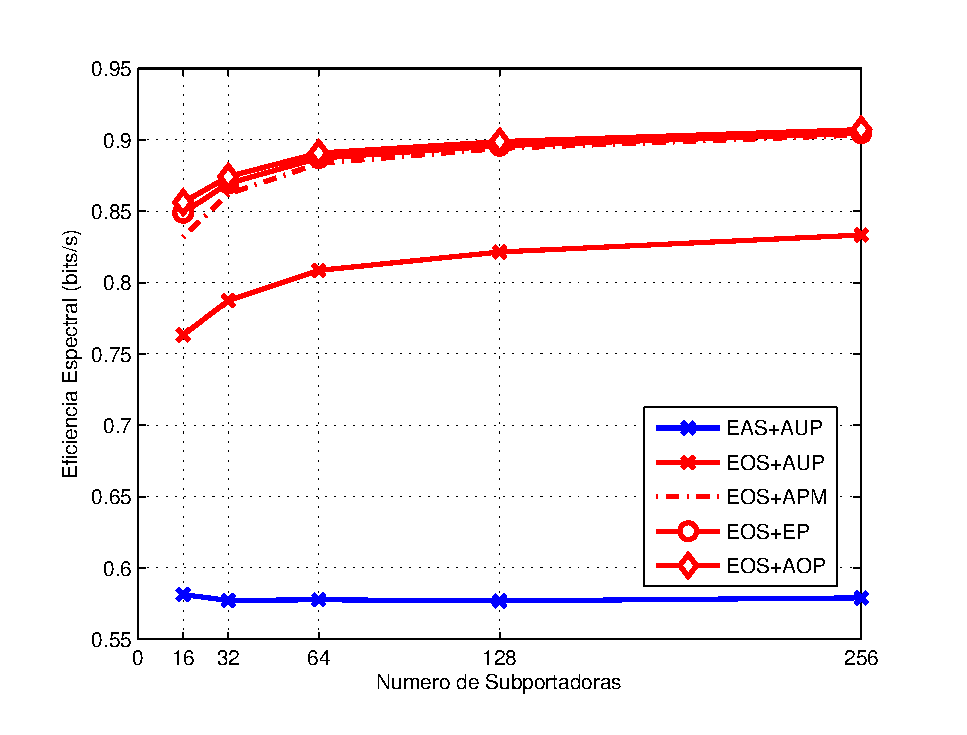
\includegraphics[width=0.6\linewidth]{../Imagens/SNxSE-5dB.eps}
     \caption{Eficiência Espectral $\times$ Número de Subportadoras em um ambiente com $\overline{\text{SNR}} = 5$~dB.}\label{fig:SNxSE-5dB}
   \end{figure}
\end{frame}

\begin{frame}{Impacto do Número de Subportadoras}
   \begin{figure}[!htb]
     \centering
     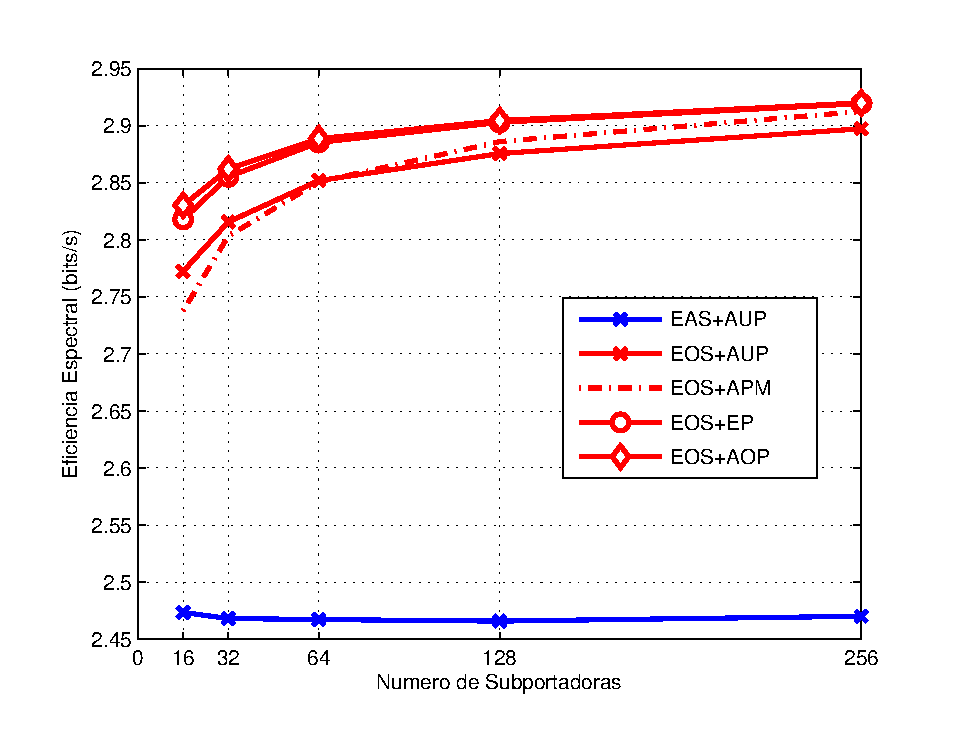
\includegraphics[width=0.6\linewidth]{../Imagens/SNxSE-20dB.eps}
     \caption{Eficiência Espectral $\times$ Número de Subportadoras em um ambiente com $\overline{\text{SNR}} = 20$~dB.}\label{fig:SNxSE-20dB}
   \end{figure}
\end{frame}

\begin{frame}{Impacto do Número de Subportadoras}
   \begin{figure}[!htb]
     \centering
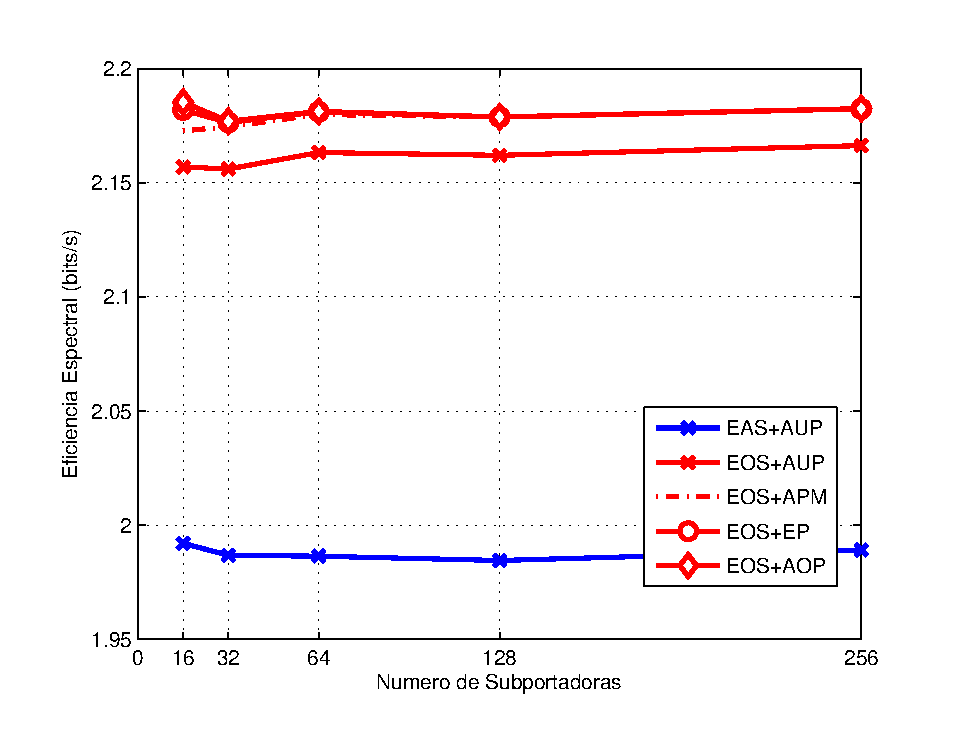
\includegraphics[width=0.6\linewidth]{../Imagens/SNxSE-Unbal-SNR.eps}
\caption{Eficiência Espectral $\times$ Número de Subportadoras em um ambiente com desbalanço de SNR.}\label{fig:SNxSE-Unbal-SNR}
   \end{figure}
\end{frame}

\begin{frame}{Impacto do Número de Subportadoras}
   \begin{bigitem}
      \item O algoritmo EOS+EP tem o melhor desempenho dentre todos os algoritmos subótimos analisados e em todos os cenários.
      \item Ao haver desbalanço de SNR, o algoritmo EOS+APM obtém seus melhores resultados.
      \item Percebemos que o maior impacto na eficiência espectral é o emparelhamento de subportadoras.
   \end{bigitem}
\end{frame}

\begin{frame}{Impacto do Ganho de Canal Médio}
   \begin{bigitem}
      \item É feito agora a variação dos ganhos de canais médios de ER-EA, avaliando a razão $E[h^r_i]/E[h^s_i]$, mantendo $E[h^s_i] = 1$.
      \item O intervalo de variação é $[0.1,5]$ e contém 20 pontos espaçados de forma logarítmica.
      \item O número de subportadoras foi mantido fixo em 64.
   \end{bigitem}
\end{frame}

\begin{frame}{Impacto do Ganho de Canal Médio}
   \begin{bigitem}
      \item Em relação à variação da razão do ganho de canal médio, foram considerados mais dois cenários possíveis:
        \begin{enumerate}[\noindent i)]
           \item Ambiente com $\overline{\text{SNR}} = 5dB$ em ambos os saltos.
           \item Ambiente com $\overline{\text{SNR}} = 20dB$ em ambos os saltos.
        \end{enumerate}
   \end{bigitem}
\end{frame}

\begin{frame}{Impacto do Ganho de Canal Médio}
   \begin{figure}[!htb]
     \centering
     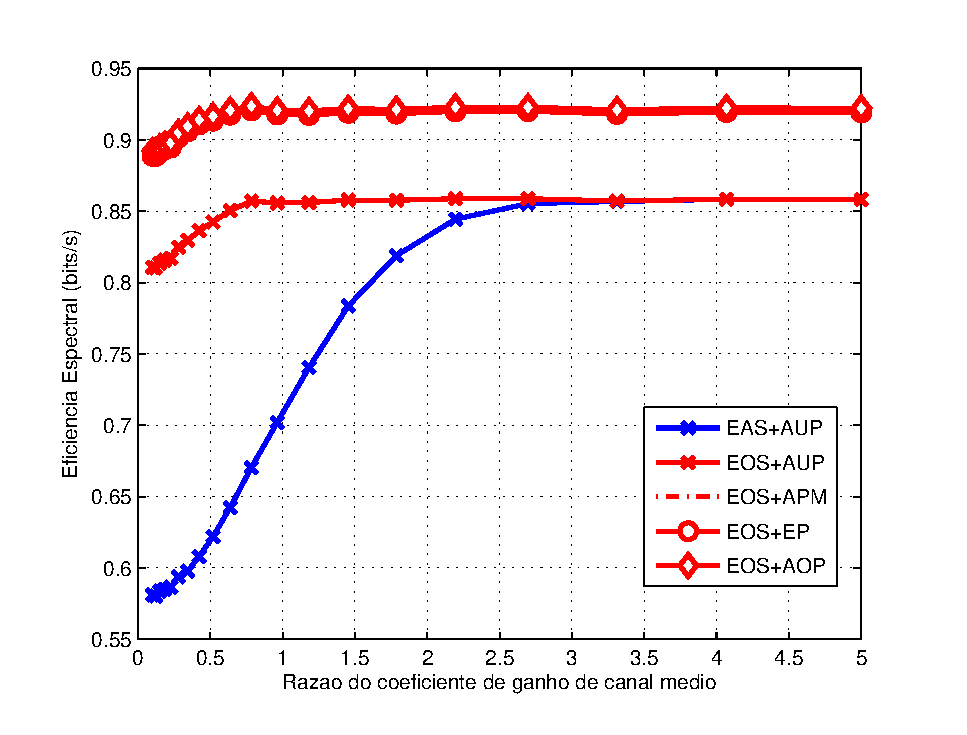
\includegraphics[width=0.6\linewidth]{../Imagens/CGxSE-5dB.eps}
     \caption{Eficiência Espectral $\times$ Razão do Ganho de Canal Médio em um ambiente com $\overline{\text{SNR}} = 5$~dB.}\label{fig:CGxSE-5dB}
   \end{figure}   
\end{frame}

\begin{frame}{Impacto do Ganho de Canal Médio}
   \begin{figure}[!htb]
     \centering
     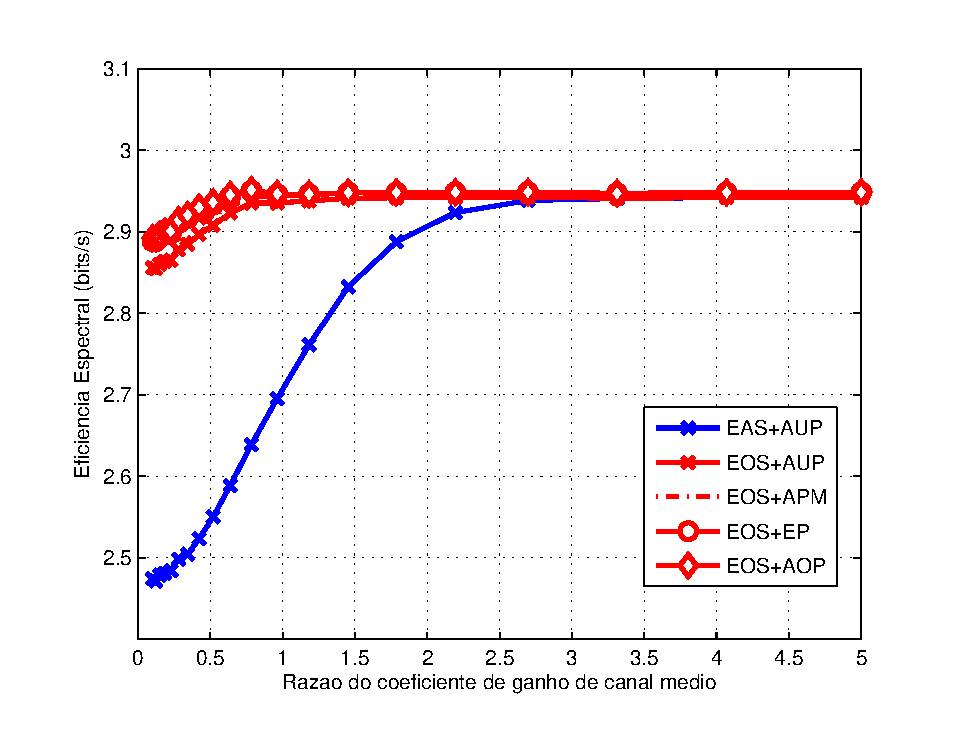
\includegraphics[width=0.6\linewidth]{../Imagens/CGxSE-20dB.eps}
     \caption{Eficiência Espectral $\times$ Razão do Ganho de Canal Médio em um ambiente com $\overline{\text{SNR}} = 20$~dB.}\label{fig:CGxSE-20dB}
   \end{figure}   
\end{frame}

\begin{frame}{Impacto do Ganho de Canal Médio}
   \begin{bigitem}
      \item É possível perceber o impacto do emparelhamento de subportadoras observando a saturação do algoritmo EAS+AUP.
      \item O algoritmo EOS+EP obtém novamente os melhores resultados dentre todos os algoritmos subótimos.
   \end{bigitem}
\end{frame}
